Generating realistic \dvpip events and simulating physics experiments are computationally intensive tasks. Personal computers can run the necessary software, but a sufficient number of simulated events would require an unacceptably long amount of time on a single device. Consequently, much effort has been devoted to the construction of computational centers and corresponding data pipelines to facilitate large scale computing efforts. 

\subsection{Scope of Computations}

    How many simulated events are needed? The simple answer is ``many''. As the number of simulated events grows, the uncertainty of the acceptance estimator $\hat{\epsilon}_{acc}$ (and other computationally derived correction factors) decreases. While simulated data are significantly less expensive than experimental data, they are not free and therefore some realistic bound must be made. As a quick heuristic, it is reasonable to perform enough simulations so as that the uncertainty of the $\hat{\epsilon}_{acc}$ is negligible compared with the other uncertainties of the measurement, or at least is non-dominant. Considering only the acceptance correction in the cross section, \eqref{eq:DVPiPCrossSection_acc_corr}

    
     \begin{equation}\labelAndRemember{eq:DVPiPCrossSection_acc_corr}
           { \frac{    d^4\sigma_{  ep \rightarrow ep'\pi^0}   } {dQ^2dx_Bdtd\phi_{\pi}} 
                =   \frac{ \textcolor{red}{ N(Q^2,x_B,t,\phi_{\pi})}} {\Lumiint \textcolor{purple}{ \Delta \Omega}}
                \frac{1}{\textcolor{correctionfactors}{\epsilon_{acc}}} = \frac{ \textcolor{red}{ N_{exp} }} {\Lumiint \textcolor{purple}{ \Delta \Omega}}  \frac{\textcolor{correctionfactors}{N_{gen}}}{\textcolor{correctionfactors}{N_{sim}}}},
     \end{equation}     

     we have the statistical uncertainty from the experimental and stimulated number of events as \eqref{eq:uncert_sum}

    \begin{equation}\label{eq:uncert_sum}
               { 
               \frac{\delta_{\sigma}}{\sigma} = \sqrt{
                \left(\frac{\delta_{N_{exp}}}{N_{exp}} \right)^2+
                \left(\frac{\delta_{N_{sim}}}{N_{sim}} \right)^2 }               }.
         \end{equation}

    %Note that this equation only discusses the uncertainties due to Nsim Nexp for illustration

    The uncertainty in \Nexp and \Nsim, $\delta_{N_{exp}}$ and $\delta_{N_{sim}}$ respectively, are given by $\sqrt{N_{exp}}$ and $\sqrt{N_{sim}}$, which assumes applicability of a Poisson distribution to the process, commonly known as ``counting statistics'' further discussed in \parencite{Knoll2000RadiationMeasurement}. We can then consider the effect of setting \Nsim = X\Nexp, where X is some multiplicative factor. The expression for the total uncertainty then can be reduced to \eqref{eq:uncert_sum_reduced}

        \begin{equation}\label{eq:uncert_sum_reduced}
               {\frac{\delta_{\sigma}}{\sigma} = \sqrt{ \left( \frac{ \sqrt{ N_{exp}} } { N_{exp}} \right)^2  +  \left( \frac{ \sqrt{ X N_{exp}} } { X N_{exp}} \right)^2     } =  \left(\frac{\delta_{N_{exp}}}{N_{exp}} \right) \sqrt{ \left(1+\frac{1}{X} \right)}}.
        \end{equation} \myequations{Relationship between \Nsim and statistical uncertainty}

    The relationship between the combined statistical uncertainty and the number of simulated datapoints is displayed graphically in \figref{fig:simulation_stats_increase}. Other uncertainties in this measurement are at the 5\%-10\% level (\secref{sec:uncertainty_analysis}) so a reasonable first-pass goal targets the statistical uncertainty due to simulation to sit at the 5\% level, corresponding to a factor X = 10 times more simulated events than experimental events. 
    
    \begin{figure}[htb]
        \centering
        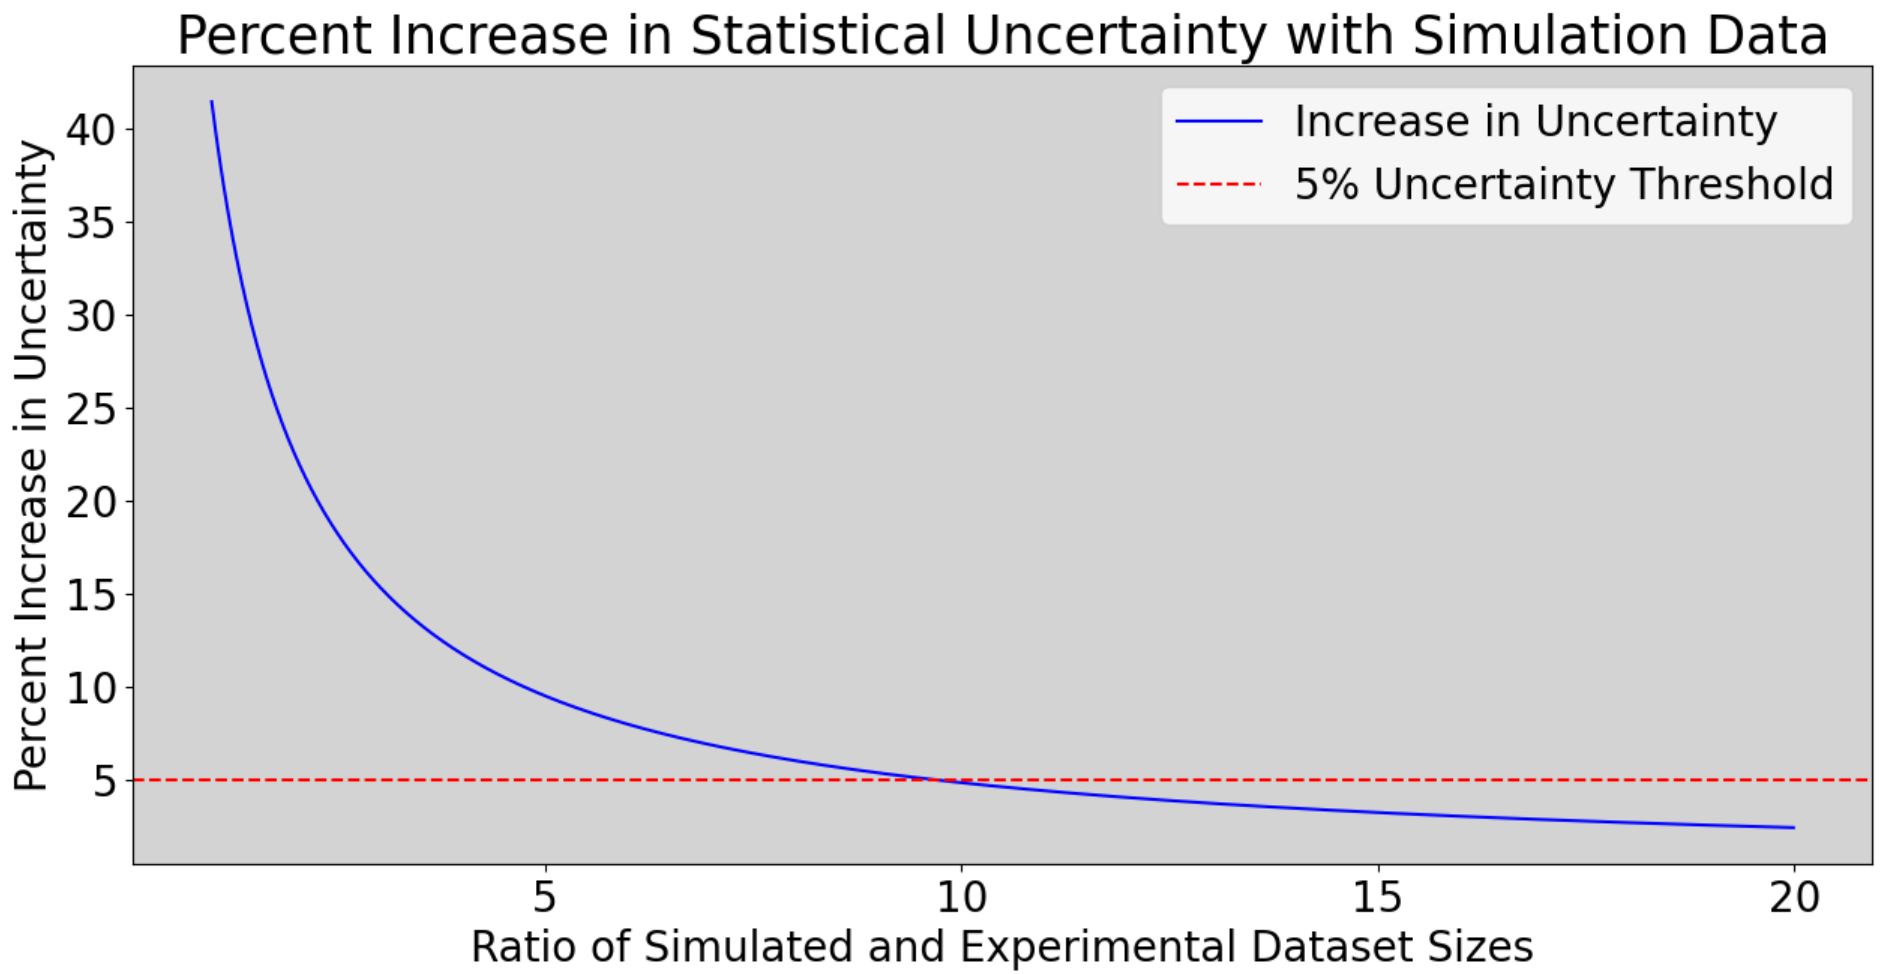
\includegraphics[width=0.8\textwidth]{Chapters/Ch3-Simulations/overview/pics/uncertainty_increase_rectangle.png}
        \caption[Comparison between Experimental and Statistical Counting Uncertainties]{Ratio of magnitudes of statistical uncertainties associated with \Nsim and \Nexp as a function of X = $\frac{N_{sim}}{N_{exp}}$. See \appref{app:f} for more details.}
        \label{fig:simulation_stats_increase}
    \end{figure}

    Preliminary analysis revealed that the total number of \dvpip events from the experimental datasets considered was approximately 500,000 ($\sim$ 200,000 from the inbending configuration, 300,000 from the outbending configuration). This corresponds to requiring $\sim$ 5 million simulated events (passing all levels of reconstruction and exclusivity cuts). The acceptance correction factor was expected to be on the order of 1/20 - 1/100, suggesting the need for several hundred million generated events to be passed through the simulation pipeline. \tabref{table:Generated_Data} displays the simulation allocation scheme implemented in this analysis, with higher statistics assigned to the nominal experiment running parameters, and additional simulations budgeted for variational studies and correction factor determination, as further discussed in \chref{Chapter:BaseAnalysis}.


    \iffalse
    \begin{table}[h]
        \centering
        \begin{tabular}{l|lccc}
            \textbf{Config.} & \textbf{Gen. Type} & \textbf{Background} & \textbf{Nevents (MM)} & \textbf{Purpose} \\ \hline
                & norad & none & 100 & Ineff. Study \\
                & norad & 50 nA & 100 & Ineff. Study / Rad. Corr \\
            In. & rad & 50 nA & 300 & Acceptance Corr. \\
                & rad & 45 nA & 100 & Systematics \\
                & rad & 55 nA & 100 & Systematics \\ \hline
                & norad & none & 100 & Ineff. Study \\
                & norad &  50 nA & 100 & Ineff. Study / Rad. Corr \\
            Out. & rad & 50 nA & 300 & Acceptance Corr. \\
                 & rad & 40 nA & 100 & Systematics \\
             & rad & 40 nA (+1.01) & 100 & Systematics \\
            \hline
            Total & - & - & 1400 & - \\
        \end{tabular}
    \caption{Data for various experimental configurations and conditions.}
    \label{table:experiments}
    \end{table}
    
    \fi
    

    \begin{table}[htb]
        \centering
        \begin{tabular}{c|ccc}
            \textbf{Configuration} & \textbf{Gen. Type} & \textbf{Background} & \textbf{Nevents (MM)} \\ \hline
                & norad & none & 100 \\
                & norad & 50 nA & 300 \\
            Inbending & rad & 50 nA & 300 \\
                & rad & 45 nA & 100 \\
                & rad & 55 nA & 100 \\ \hline
                & norad & none & 100 \\
                & norad &  50 nA & 300 \\
            Outbending & rad & 50 nA & 300 \\
                 & rad & 40 nA & 100 \\
             & rad & 40 nA (+1.01) & 100 \\
            \hline
            Total & - & - & 1800 \\
        \end{tabular}
    \caption[Distribution of Generated Events by Configuration]{Number of events generated for various experimental configurations and conditions. \tabref{table:simulated_data} shows this distribution after simulation, reconstruction, and exclusivity cuts.}
    \label{table:Generated_Data}
    \end{table}


    Optimization studies showed that the most computationally efficient batching scheme was to process batches of 10K events to GEMC at a time, which was the bottleneck in the simulation pipeline at 4.5 - 5 hours per job. The non-radiative (radiative) event generator requires 10 minutes (100 minutes) to produce 10K events, and further processing upon completion of GEMC requires $\sim$ 10 minutes per 10K events. This totals $\sim$ 5 hours (6 hours) per 10K events, corresponding to nearly 1 million core-hours for the required total number of simulations, which would take 8 years of continuous running on a single, high-end, 16 core computer. Instead, computing clusters at MIT, JLab, and around the globe were utilized to realize these computational efforts in a much more reasonable timeframe. 
    


    \iffalse
    \begin{table}[h]
        \centering
        \begin{tabular}{c|ccc}
            \textbf{Configuration} & \textbf{Gen. Type} & \textbf{Background} & \textbf{Nevents (MM)} \\ \hline
                & norad & none & 5 \\
                & norad & 50 nA & 5 \\
            Inbending & rad & 50 nA & 15 \\
                & rad & 45 nA & 10 \\
                & rad & 55 nA & 10 \\ \hline
                & norad & none & 10 \\
                & norad &  50 nA & 10 \\
            Outbending & rad & 50 nA & 30 \\
                 & rad & 40 nA & 10 \\
             & rad & 40 nA (+1.01) & 10 \\
            \hline
            Total & - & - & 1400 \\
        \end{tabular}
    \caption[Distribution of Simulated Events by Configuration]{Number of simulated events for various experimental configurations and conditions.\tabref{table:Generated_Data} shows the corresponding number of generated events per distribution. \textcolor{red}{\textbf{NOTE: Values in this table are placeholders and need to be updated with final figures}}}
    \label{table:simulated_data}
    \end{table}

    \fi



    
    \todo{find some way to include the distribution of ambient radiation (cememnt, etc) - Knoll 767 -  into thesis appendix - include discussion of background merging - not an issue at these scales}


\subsection{MIT Tier 2 and High Throughput Computing}

    The primary computing center utilized for this analysis effort was the MIT Tier 2 cluster, located at the MIT Bates Research and Engineering Center in Middleton, MA, which has 1,088 cores dedicated to CLAS12 computing \figref{fig:BatesComputing}.  Also used for this work was the Massachusetts Green High Performance Computing Center (\href{https://www.mghpcc.org/}{MGHPCC}) in Holyoke, MA. MIT Earth and Planetary Science provides access to these nodes through their \href{https://engaging-ood.mit.edu/pun/sys/dashboard}{Engaging} system, while the MIT Tier 2 cluster is accessible via the \href{https://submit.mit.edu/}{subMIT} system, which also grants users access to a number of other (non-dedicated) computing clusters.

    


    %1,088 cores dedicated to CLAS computing. I believe this means we have 24 hours per day * 1088 cores = ~ 26K core hours per day dedicated   
    %The Bates Laboratory center consists of 71 water-cooled racks, each of which can supply up to 12 kW of power and cooling, and a high-speed 100 Gb/s network link to campus. It uses about 500 kW of power to operate and have 20 petabytes of storage at present.


    \begin{figure}
        \centering
        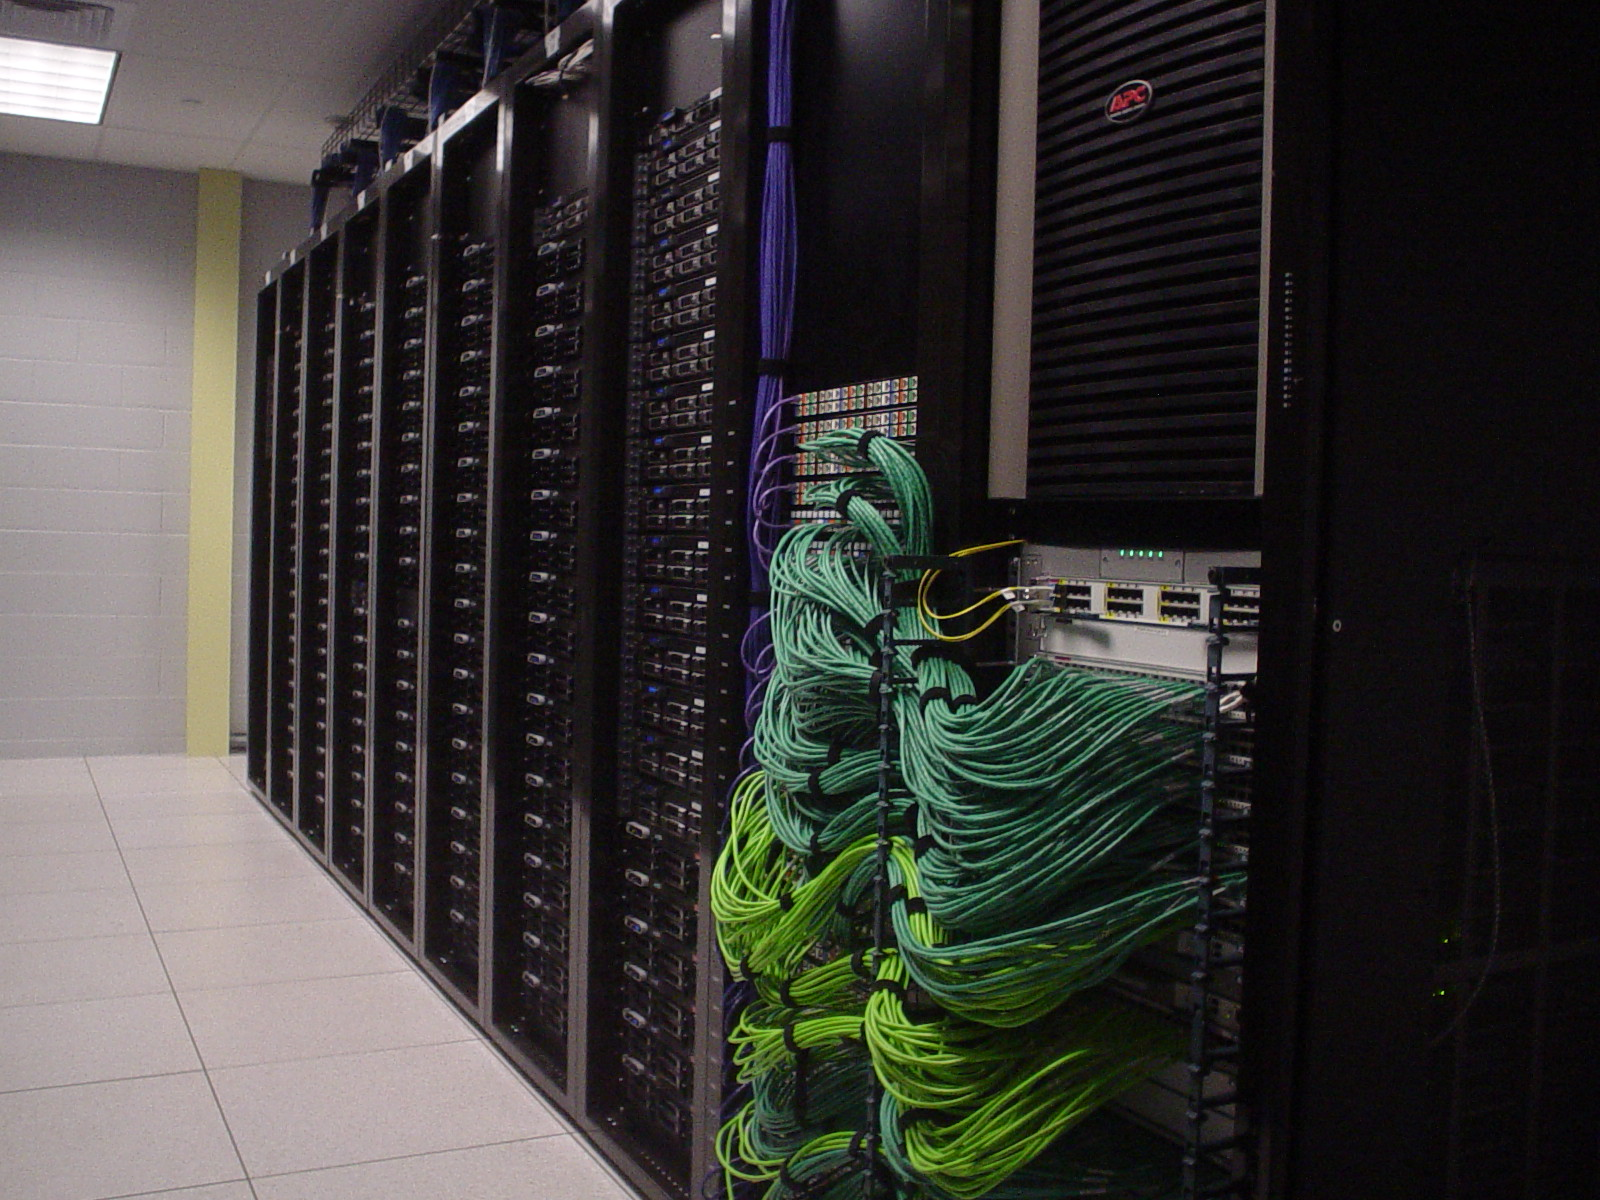
\includegraphics[width=0.8\textwidth]{Chapters/Ch3-Simulations/overview/pics/Bates_Tier2.jpg}
        \caption[MIT Tier 2]{MIT Tier 2 computing racks at MIT Bates. Image courtesy of E. Ihloff}
        \label{fig:BatesComputing}
    \end{figure}


    
    %and is, which is a larger computational framework that additionally provides access to other computing centers,



    %SUBMIT:     1 TB of free storage per user,     100s of cores and GPUs available interactively and through Slurm     Access to OSG, CMS T3 and T2, LQCD Cluster, and EAPS


    More broadly, the Open Science Grid (OSG) \parencite{OSG2006OSG} \parencite{Sfiligoi2009TheGlideinWMS} \parencite{Pordes2007TheGrid} was leveraged to gain access to dozens of computing clusters around the world. OSG is an organizational system allowing users to utilize idling resources at more than 100 participating institutions, facilitating more than a billion core-hours of computation per year. 

    A significant endeavor in this work was constructing a software bridge connecting the CLAS12 experiment and these computing resources. The effort was realized as the \href{https://gemc.jlab.org/web_interface/index.php}{CLAS12 Simulation Submission Portal} \parencite{Ungaro2020CLAS12Framework}, which established the database back-end, user-friendly front-end \figref{fig:clas12_sub_portal}, and appropriate connection services to interact efficiently with these clusters. 
      
    \begin{figure}[H]
        \centering
        \newlength{\imageheight}
        \settoheight{\imageheight}{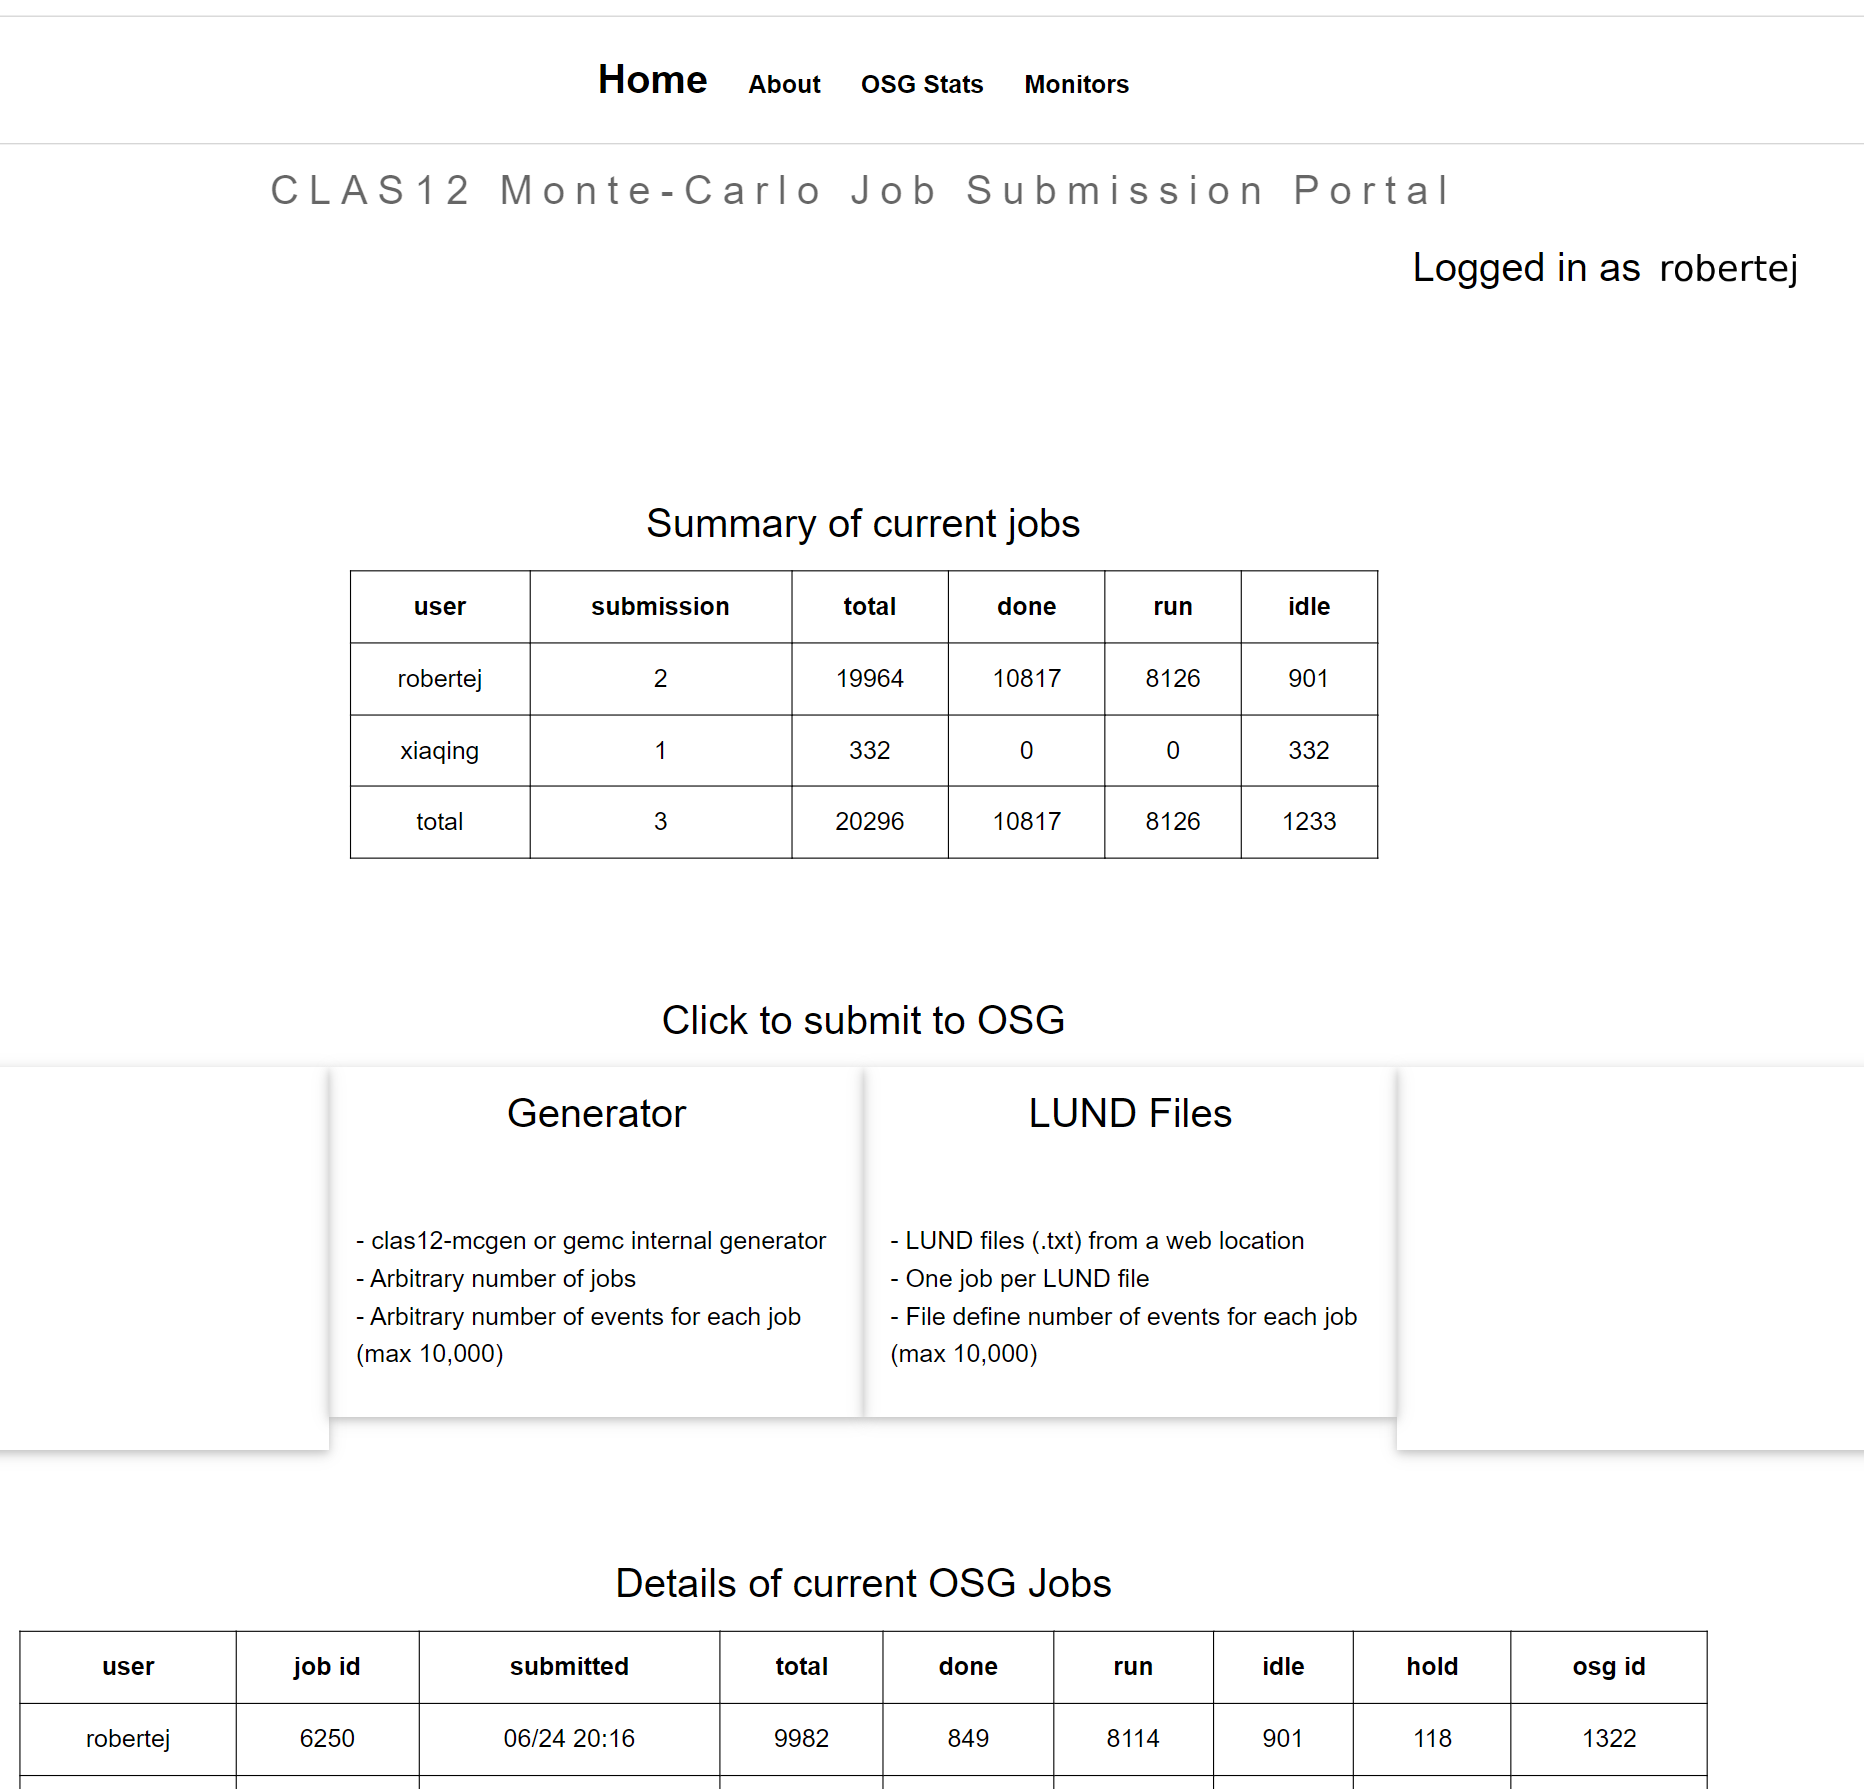
\includegraphics[width=0.5\textwidth]{Chapters/Ch3-Simulations/overview/pics/websub_start_narrow_new.png}}
        \subfloat[CLAS12 Submission Portal Main Page]{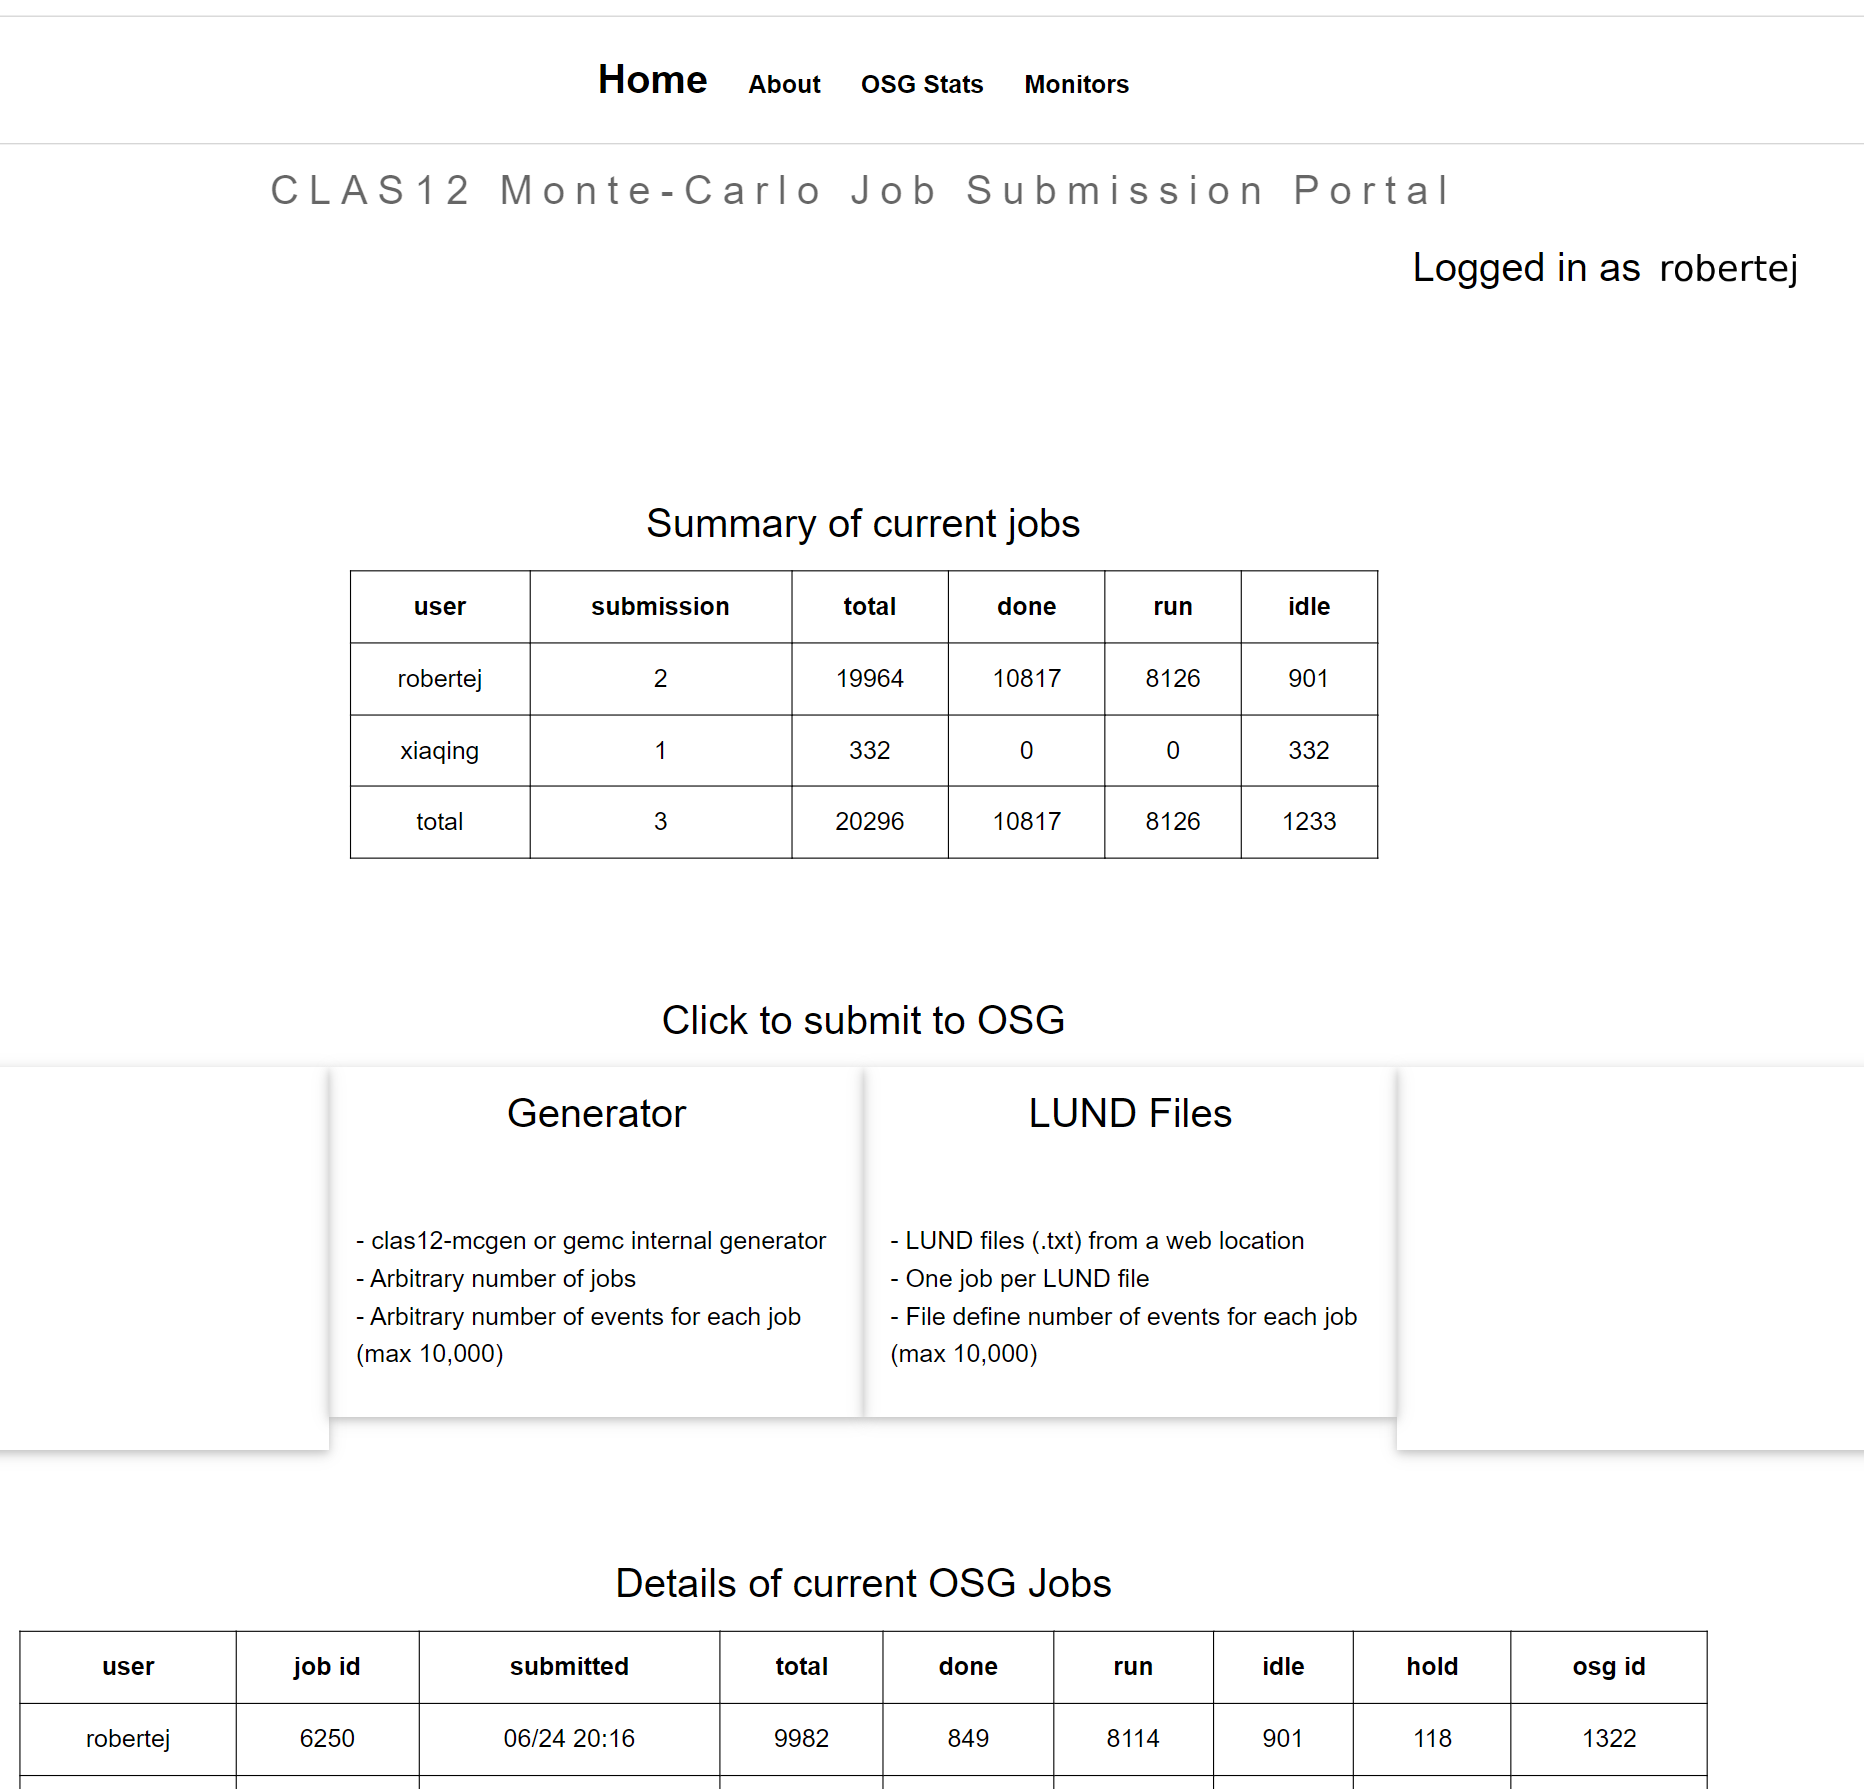
\includegraphics[width=0.5\textwidth]{Chapters/Ch3-Simulations/overview/pics/websub_start_narrow_new.png}}
        \hfill
        \subfloat[Simulation Sample Webform]{\raisebox{\dimexpr\imageheight-\height}{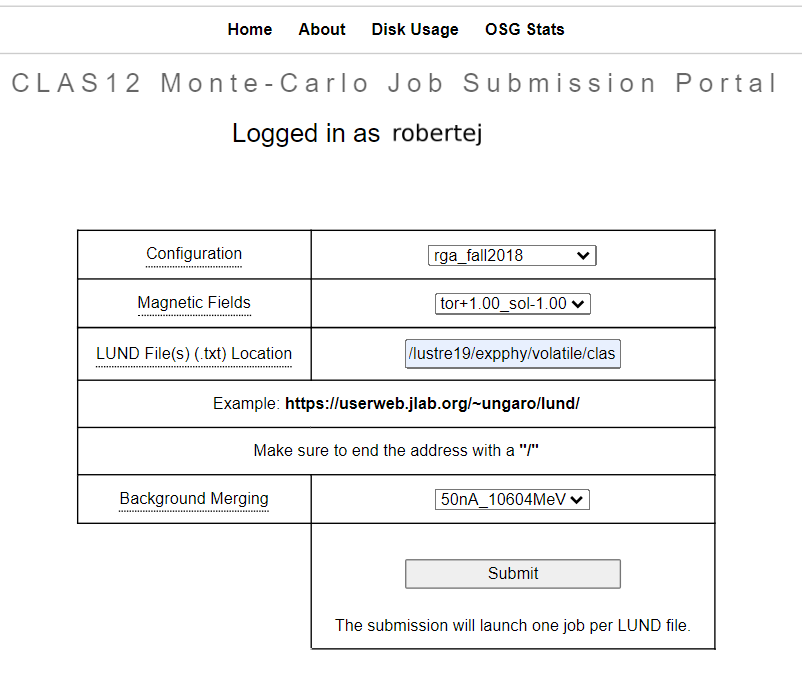
\includegraphics[width=0.45\textwidth]{Chapters/Ch3-Simulations/overview/pics/websub_lund.png}}}
        \caption[CLAS12 Simulation Submission Portal]{The CLAS12 Simulation Submission Portal, designed to facilitate efficient high-throughput simulations using a variety of generators and experimental configurations.}\label{fig:clas12_sub_portal}
    \end{figure}

    The system is capable of using any event generator on the CLAS collaboration list of \href{https://github.com/JeffersonLab/clas12-mcgen}{officially approved generators} or by passing any internet-accessible folder location of generated event files conforming to the \href{https://gemc.jlab.org/gemc/html/documentation/generator/lund.html}{LUND} standard. As of July 2023, the aao\_gen generators were not yet recognized as officially supported, so event generation had to occur independently of this system, although work is ongoing to recieve offical status. Inferfacing with computing nodes is facilitated through use of Simple Linux Utility for Resource Management (SLURM) \parencite{Yoo2003SLURM:Management} and High Throughput Computing - HTCondor \parencite{HTCondorTeam2023HTCondor} protocols. The system has been succesful, facilitating 85.2 million core-hours of CLAS12 simulations over 2021-2022 as shown in \figref{fig:monthly_hours}.
       
    
    \begin{figure}
        \centering
        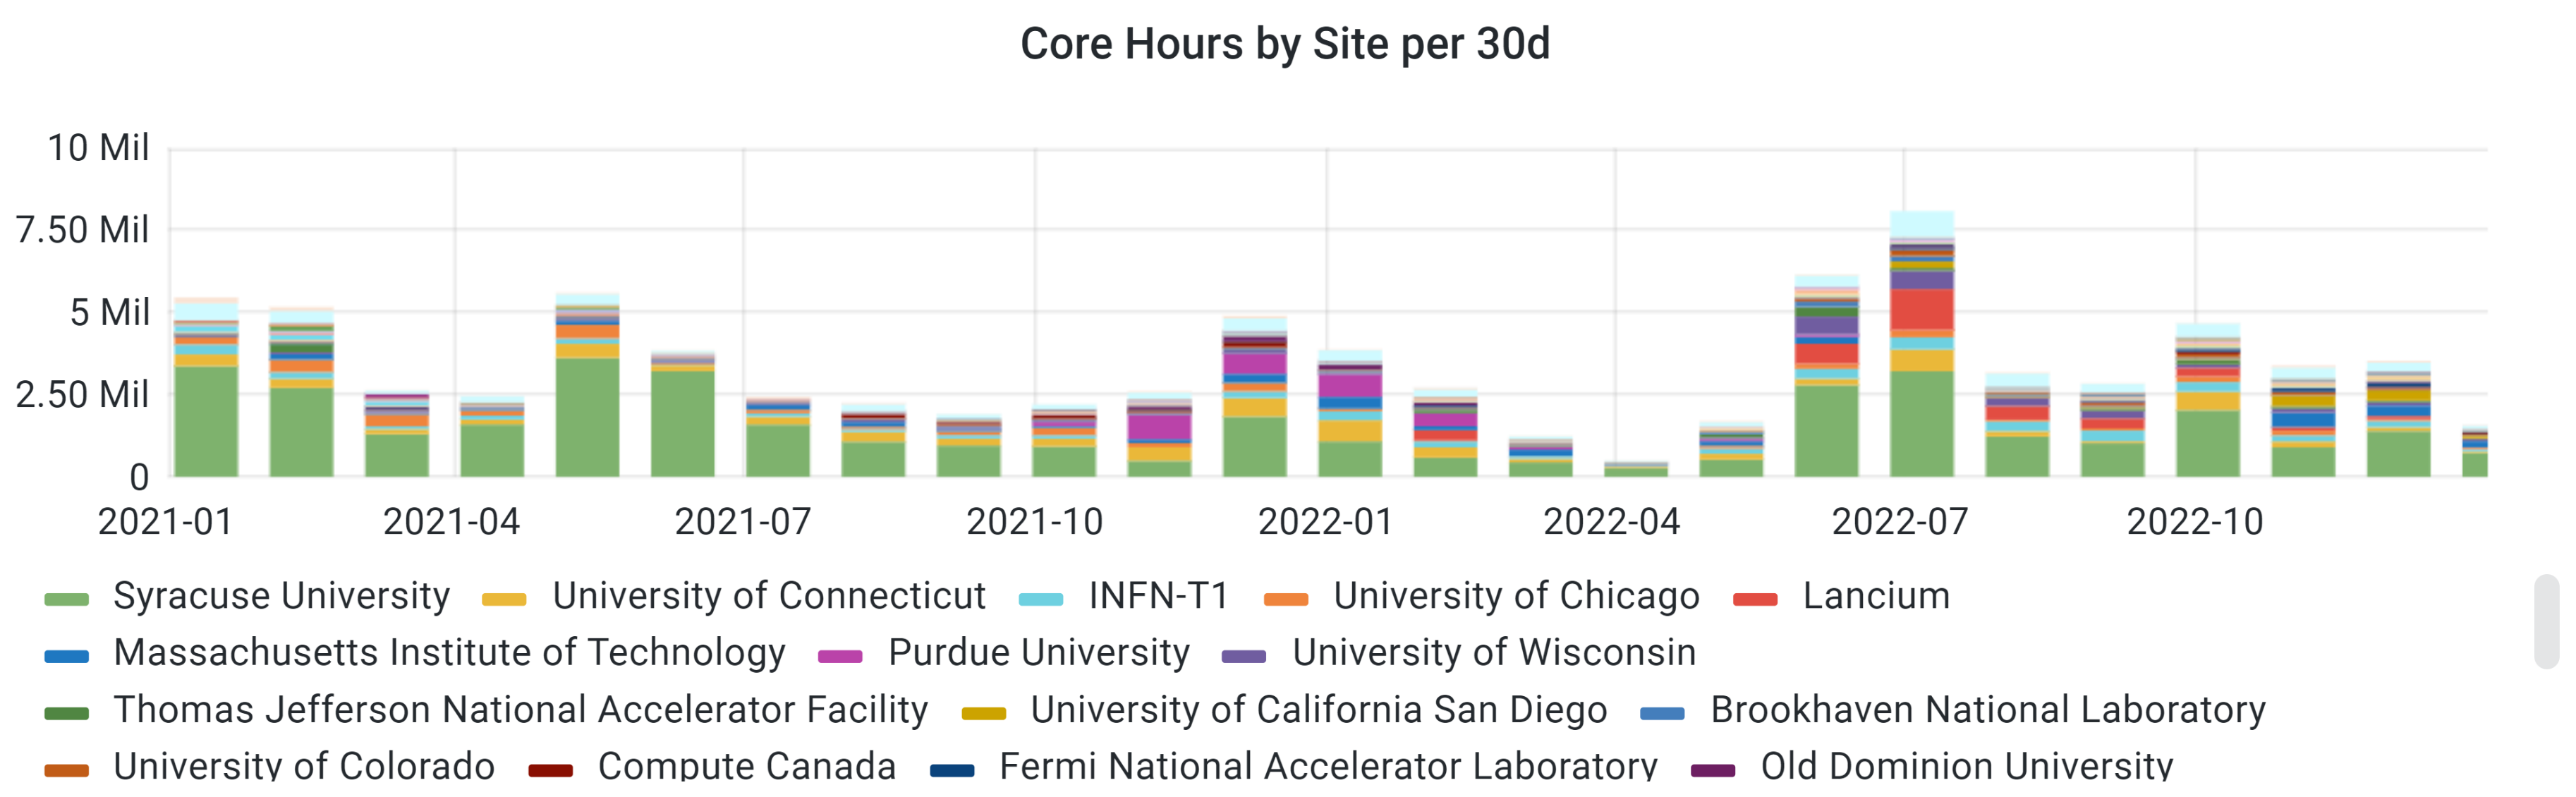
\includegraphics[width=0.99\textwidth]{Chapters/Ch3-Simulations/overview/pics/core_hours_2021-22.png}
        \caption[Monthly Core-Hours Utilized at Various Computing Clusters]{Monthly core-hours used for CLAS12 simulations in 2021-22. The portal facilitated 85.2 million core-hours of simulations over the past 2 years.}
        \label{fig:monthly_hours}
    \end{figure}

    Finally, files can be transferred easily from computing clusters to local/personal machines through the use of \href{https://www.globus.org/}{Globus} \parencite{Allen2012SoftwareScientists} \parencite{Foster2011GlobusServices}, or directly through use of ssh protocols. The complete data pipeline for simulations used in this analysis is shown in \figref{fig:simulation_workflow}.


    \begin{figure}
        \centering
        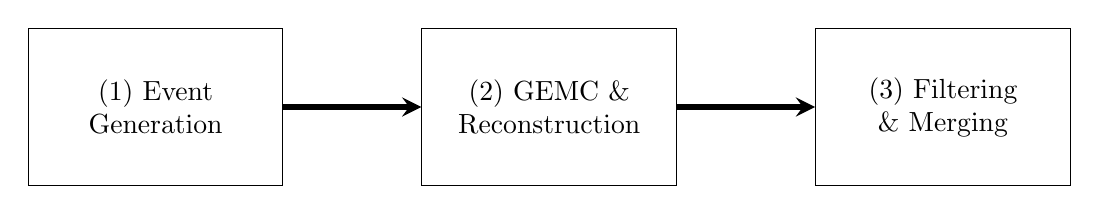
\begin{tikzpicture}[
            box/.style={rectangle, draw, minimum size=2cm, text width=3cm, align=center},
            arrow/.style={->, >=stealth, line width=2pt},
        ]
        
        \node[box] (event) at (0,0) {(1) Event \\ Generation};
        \node[box] (gemc) at (5,0) {(2) GEMC \& \\ Reconstruction};
        \node[box] (filter) at (10,0) {(3) Filtering \& Merging};
        
        \draw[arrow] (event) -- (gemc);
        \draw[arrow] (gemc) -- (filter);
        
        \end{tikzpicture}
        \caption[Event Simulation Pipeline]{Event simulation pipeline. (1) Events are generated using aao\_gen on either MIT Tier 2, MGHPCC, or JLab's SciComp nodes. (2) Events are submitted through the CLAS12 Submission Portal to run on dedicated or idling resources to the GEMC \& CLAS12 event reconstruction suite. (3) Simulated events are returned to JLab's computing nodes, where they are further filtered as discussed in \secref{sec:filtering} and transferred to local computers for analysis.}
        \label{fig:simulation_workflow}
    \end{figure}


    

    \todo{WHERE IS THE JLAB IFARM INFO?}
   
    
    %It includes in addition, a CMS HI simulation and analysis facility, an LHCb Tier-2 computing center, a Hadronic Physics computing center and various smaller contributions. Presently it is located at Bates in Middleton MA.

    %distributed high throughput computing systems - 





    




    
    
    
    %volatile work
    %To cancel all jobs:
    %scancel -u robertej
    
    %To view all jobs:
    %squeue -u robertej

    
    %local of disk utilization statistics: https://clasweb.jlab.org/clas12offline/disk/work/users.html
    




    %is an intercollegiate high-performance computing facility - joint venture between Boston University, Harvard, MIT, Northeastern, and the University of Massachusetts system. - 300 nodes, 10K CPUs, 

 

    
    
    


